The Quantum Approximate Optimization Algorithm (QAOA) is a class of hybrid quantum-classical approximate algorithms which can tackle combinatorial optimization problems \cite{farhi2014quantum, alam2019analysis}.
QAOA combines the preparation of a quantum state and the properties of superposition with classical optimization.
As is in the name, it is also an approximate algorithm thus it does not necessarily give the optimal solution (the actual partition with MaxCut in our case) but gives an approximation of such a solution.

At the current stage of development of Quantum Computing infrastructure, called \textit{Noisy Intermediate Scale Quantum} era or NISQ era, QAOA are of particular interest.
There has been considerable interest already in developing use cases within the limits of currently available quantum computers as well as projecting the kind of quantum advantage we might be able to achieve in near term \cite{Guerreschi_2019}.
As has been shown in contemporary works \cite{8957201} as well, we also look at the limitations of QAOA using the currently available quantum computers.

Nevertheless, QAOA remains a very prominent line of thought regarding new quantum algorithms and has a wide applicability across different fields.
It can be used to solve problems in academia \cite{Bengtsson_2020}, in logistics \cite{Vikst_l_2020}, finance etc.

In this project, we look at one combinatorial optimization problem, namely the MaxCut problem as stated earlier.
We analyse the working of the algorithm in an ideal case.
We also employ simple noise models and see how the presence of noise affects the performance of the algorithm.
Further, we implement the algorithm on actual hardware backend and analyse the performance and discuss the limitations of the noisy systems we currently have.

%%%%%%%%%%%%%%%%%%%%%%%%%%%%%%%%%%%%
\section{The algorithm}

As described above, the function that we want to maximize is $C(z)=\sum_{k=1}^m C_k(z)$, with $m=|E|$ being the number of edges in the graph.
Here, $z=z_1z_2\cdots z_n$ and $z_i\in \{0,1\}$ based on which node is in which subset.
Thus, here, we encode the information about the subset a particular node belongs to by $0$ and $1$ unlike $1$ and $-1$ as discussed in last section.
$C_k \in \{0, 1\}$ based on the string $z$. It tells us if the $k^{th}$ edge is being cut or not by the partition denoted by the string $z$.
Our aim is to find the string(s) $z$ that give us the maximum value of $C$.

Firstly, we need to convert this (thus far) classical problem into a quantum problem. Thus, the string $z$ which denotes a particular partition of the nodes, translates to the quantum state $\ket{z}$.\\
To illustrate this, the partition shown in the figure \ref{fig:GraphCut}, would be denoted by the classical string $z = 01101$ and subsequently, in the quantum state $\ket{01101}$.
Thus, each of the basis state would denote a particular partition of the nodes.

Further, the cost function that we defined above and which we want to maximize, can then be represented as an operator.
We define it such that acting on any basis state (each of which now denotes a partition), it gives back the same basis state but multiplied with the the cost $C(z)$ of that basis state.
Thus, the basis states are the eigenstates with he cost as their corresponding eigenvalues. This can be expressed as
\begin{equation}
    \hat{C}\ket{z}= \sum_{k=1}^m \hat{C}_k\ket{z} = c(z)\ket{z}
    \label{equation:cost_op}
\end{equation}

For the operator $C$, there will be a specific value $c'=c(z')\geq c(z),\forall z\neq z'$ which will be the solution of our maximization problem.
For any general state $\ket{\psi}=\sum_{z \in\{0,1\}^n}a_z\ket{z}$, we can construct the expectation value of the cost function as:
\[
    \left\langle C\right\rangle =\bra{\psi}\hat{C}\ket{\psi} = \sum_{z \in\{0,1\}^n}c(z)|a_z|^2
\]
Thus, to find an approximate solution, we try to find $\ket{\psi}$ that maximizes $\langle C \rangle$

Say the actual MaxCut partition is $z^*$, then, we want to get $\ket{\psi} = \ket{z^*}$.
In that case, $\langle C \rangle = C_{max}$.
But in general, we don't know how to find $C_{max}$ efficiently.
Thus, what we do is we try and get $\langle C \rangle$ as close to $C_{max}$ as possible.
In other words, we try to get $\ket{\psi}$ such that the amplitude(s) of $\ket{z^*}$ is very high.

As a metric of performance, we define the approximation ratio denoted by $r$ and defined as
$$r = \frac{ \langle C \rangle }{C_{max}} $$
Having established our goal to get a $\ket{\psi}$ with high amplitudes for $\ket{z^*}$, let us define the quantum operators that we use.
%%%%%%%%%%%%%%%%%%%%%%%%%%%%%%%%%%%
\subsection{First step: $U_C(\gamma)$}
Firstly, we define a Hamiltonian called the \textit{Cost Hamiltonian} and we denote it by $H_C$.
This is essentially the function $C$ that we defined earlier.
Thus, it can be written as

\[
    H_C = \sum_{k=1}^m C_k = \sum_{z \in \{0, 1\}^n}C(z)\ket{z}\bra{z}
\]
As we can see it is the same operator that we defined in \ref{equation:cost_op} and it has the same properties.
Using this Hamiltonian, we define a Unitary operator $U_C(\gamma)$ in the following way:
$$U_C(\gamma) = e^{-i \gamma H_C}$$
Thus, $U_C$ is a parametric operator, parameterised by the real number $\gamma$.

Now let's see what is the action of this operator on a general state $\ket{\psi}$
\[
    U_C(\gamma)\ket{\psi}= U_C(\gamma)\sum_{z \in\{0,1\}^n} a_z\ket{z} = \sum_{z \in\{0,1\}^n} a_z e^{-i\gamma C(z)} \ket{z}
\]
Thus, all basis states get a phase depending on the cost of the partition corresponding to that state and $\gamma$.
%%%%%%%%%%%%%%%%%%%%%%%%%%%%%%%%%%%%
\subsection{Second step: $U_B(\beta)$}
The amplitudes change, however, since the only change is in the complex phases of the states, the probabilities for each state are same as before applying the operator $U_C$ and likewise, the expectation values have not changed either.

Having changed the relative phases of the states, we need to operate with an operator that now mixes them, that is, causes a superposition between these states.
To achieve this, as earlier, we first define an Hamiltonian and call it the \textit{Mixing Hamiltonian}.
We define it as following:
\[
    H_B=\sum_{k=1}^n\sigma_k^x= \sigma_1^x\otimes \mathbb{I}^{\otimes(n-1)} + \mathbb{I} \otimes \sigma_2^x \otimes \mathbb{I}^{ \otimes(n-2)}+ \cdots + \mathbb{I}^{\otimes(n-1)} \otimes \sigma_n^x
\]
Again using this Hamiltonian, we define a unitary $U_B(\beta)$ as
$$U_B(\beta)= e^{-i\beta H_B}$$
As earlier, $U_B(\beta)$ too is a parametric operator that is parameterised by real number $\beta$.

To see the action of this operator, we write $U_B(\beta)$ as
\[
    U_B(\beta)= e^{-i\beta H_B} = e^{-i\beta\sum_{k=1}^n \sigma_k^x} = \prod_{k=1}^n e^{-i\beta \sigma_k^x}
\]
Recalling the definition of the $x$-rotation operator $R_x(\theta)=e^{-i\frac{\theta}{2}\sigma^x}$, with $\theta\in [0,2\pi]$, it becomes clear that the operator $U_B(\beta)$ can be written as:
\[
    U_B(\beta)= R_x^{\otimes n}(2\beta)\quad\text{with }\beta\in [0,\pi]
\]
Which is actually a rotation about X for each qubit by an angle $2\beta$.

The combined effect of applying $U_C(\gamma)$ followed by $U_B(\beta)$ is to first give a complex phase to all the states (which depends on the cost and the parameter $\gamma$) followed by applying an X rotation (which depends on the parameter $\beta$) for all qubits.\\
Thus, all the states will mix and how exactly they mix is controlled by $\gamma$ and $\beta$.
We try and tweak these parameters such that this mixing happens in such a way that the amplitude of the states with low cost falls (they interfere destructively) and the amplitudes of the states with higher cost rises (they interfere constructively).

\subsection{Building the operators}
Having defined the operators mathematically, it is instructive to look at how we implement the operators.

From the definition and action of $U_B(\beta)$ as indicated in the previous subsection, it is rotation about X axis by an angle $2\beta$ for each qubit. Thus, it can be implemented using $n$ single qubit rotations where $n$ is the number of qubits (i.e. the number of nodes). Thus,

$$U_B(\beta)=\prod_{i=1}^{n} R_{Xi}(2\beta)$$

Now, looking at $U_C(\gamma)$, and the definition of $H_C$ and the equations \ref{g_def} and \ref{C_def} along with the fact that $\ket{z}$ denotes the partitions, we define:

$$H_C = \sum_{(jk) \in E} \frac{1}{2}(\mathbb{I}- Z_j Z_k)$$
The implementation of $U_C(\gamma)$ would then translate to
\[U_C (\gamma) = \prod_{(i,j) \in E} CR_Z_{i,j}(-2\gamma)R_{Zi}(\gamma)R_{Zj}(\gamma)\]
Where $i$ and $j$ are the nodes at the end of the edge. $CR_Z_{i,j}(-2\gamma)$ is a controlled rotation around $Z$ by angle $2\gamma$, and $R_Z_{i}(\gamma)$ is rotation about $Z$ by angle $\gamma$ for qubit $i$. We would have to apply this combination for each edge in $E$.

To see the implementation for a simple graph, consider a regular 3-node graph. The graph is as shown in figure \ref{fig:triangle}.

\begin{figure}[h]
    \centering
    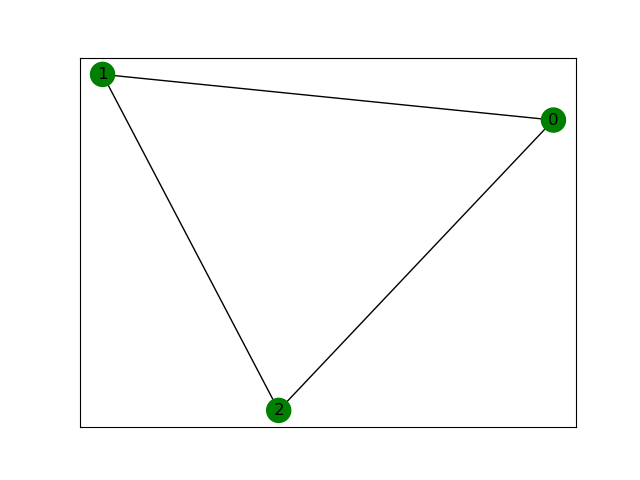
\includegraphics[scale=0.5]{images/triangle.png}
    \caption{A regular 3-node graph.}
    \label{fig:triangle}
\end{figure}

To implement QAOA for this graph, we would have to apply the following gates as shown in figure \ref{fig:3ncircuit}

\begin{figure}[h]
\begin{center}
    \begin{quantikz}
        \lstick{$\ket{+}$}  & \ctrl{1}\gategroup[wires=3,steps=6,style={inner sep=6pt}]{$U_C$} & \gate{R_Z(\gamma)} & \qw & \qw & \ctrl{2} &  \gate{R_Z(\gamma)} &\qw & \gate{R_X(2\beta)}\gategroup[wires=3,steps=1,style={inner sep=6pt}]{$U_B$} &\meter{} &\cw \\
        \lstick{$\ket{+}$}  & \control{} & \gate{R_Z(\gamma)} & \control{} & \gate{R_Z(\gamma)} & \qw & \qw &\qw &\gate{R_X(2\beta)} & \meter{} & \cw\\
        \lstick{$\ket{+}$}  & \qw & \qw  & \ctrl{-1} & \gate{R_Z(\gamma)} & \control{} & \gate{R_Z(\gamma)} &\qw &\gate{R_X(2\beta)} & \meter{} & \cw
    \end{quantikz}
%    \includegraphics[width=1\linewidth]{circuit.png}
    \caption{Circuit for the 3-n regular graph with the final measurement in the computational basis}
    \label{fig:3ncircuit}
\end{center}
\end{figure}


Note that the circuit on figure \ref{fig:3ncircuit} is not optimal. Since all gates commute, the circuit could be compiled with many less gates. Nevertheless, for the sake of simplicity, we will stick to this ansatz as this allows to easily generalize for different graphs.

It would be insightful to talk about the particular structure of $U_B$ or rather its relation to $U_C$.\\
Note that here, the gates in $U_C$ and those in $U_B$ do not commute.
By extension, $U_C$ and $U_B$ themselves do not commute.
This is an important feature.

To illustrate this, let us see what would happen in case we defined $H_B$ and by extension $U_B$ in the same manner but instead of having the rotation about X axis, we rotated about Z axis.
First, it is clear that in that case, $U_C$ and $U_B$ would commute. But why is this undesirable?

From our discussion earlier, we know that $U_C$ applies phase to all states, thus it does not change the probabilities.
If $U_B$ were to commute with it, then that means, $U_C$ and $U_B$ would have the same eigenbasis.
And in that case, applying $U_B$ to the eigenstates of $U_C$ (which are the standard basis states), one would get
$$U_B(\beta)\ket{z} = b(z)\ket{z}$$
since these are also the eigenstates of $U_B$. And since, $U_B$ is a unitary matrix, the eigenvalues are all of unit magnitude. Thus, applying $U_B$ is same as applying some phase.

All of this would mean that the amplitudes of the states change but they change only in terms of the phase they have.
And thus, the probabilities of these states are unchanged.\\
This means, $\langle C \rangle$ which we want to maximise, never changes, no matter what values of $\gamma$ and $\beta$ we choose.
Thus, it is crucial that $U_B$ and $U_C$ do not commute since the only purpose of $U_B$ is to mix the states (thus the name \textit{Mixing Hamiltonian} for $H_B$) and that would not be possible if they commute.
This means, we could choose rotations about $Y$ instead of $X$ for $H_B$ but not about $Z$ or anything that commutes with $U_C$ 

\section{Workflow}

Having defined the necessary operators, we have a look at the algorithm now.
We start with a state that is equal superposition of all states. Then we start with:

\[\ket{\psi}=H^{\otimes n}\ket{0}^{\otimes n} = \frac{1}{\sqrt{2^n}}\sum_{z \in\{0,1\}^n}\ket{z}\]

On this initial state, we apply $U_C(\gamma)$ followed by $U_B(\beta)$.
Let us say, we do this for $p$ times.
Thus we have $2p$ parameters, i.e, $p$ values of $\gamma$ and $p$ values of $\beta$.
From here on, we call one application of $U_C$ followed by $U_B$ a layer.
Thus, we here have $p$ layers.

After applying the unitary transformations, we measure the qubits in standard basis to get the state $z$ and from that, we get the cost for that state i.e, $C(z)$.\\
Thus, the circuit can be represented as in the figure \ref{fig:General_QC} below

\begin{figure}[h]
    \centering
    \begin{quantikz}
        \lstick[wires=4]{$\ket{0}^{\otimes n}$} & \gate{H} & \gate[wires=4]{U_C(\gamma_1)}\gategroup[4,steps=2,style={dashed,
        rounded corners,fill=blue!20, inner xsep=2pt},
        background,label style={label position=below,anchor=
        north,yshift=-0.2cm}]{{$1^{st}$ layer}} & \gate[wires=4]{U_B(\beta_1)}& \ \ldots\ \qw & \gate[wires=4]{U_C(\gamma_p)}\gategroup[4,steps=2,style={dashed,
        rounded corners,fill=blue!20, inner xsep=2pt},
        background,label style={label position=below,anchor=
        north,yshift=-0.2cm}]{{$p^{th}$ layer}} & \gate[wires=4]{U_B(\beta_p)}& \meter{} & \cw\rstick[wires=4]{Measure\\results}\\
        & \gate{H} & & & \ \ldots\ \qw & & &\meter{} & \cw \\
        &\wave & & & & & & & &\\
        & \gate{H} & & & \ \ldots\ \qw & & &\meter{} & \cw 
    \end{quantikz}
    \caption{This is a general representation of the quantum circuit for $n$ qubits and $p$ layers.}
    \label{fig:General_QC}
\end{figure}



We start with arbitrary values of the $2p$ parameters for the operators.
The state just before measurement is denoted as $\ket{\gamma, \beta}$, which would be:
\[
    \ket{\gamma,\beta} = U_B(\beta_p)U_C(\gamma_p)\cdot\cdot\cdot U_B(\beta_2)U_C(\gamma_2)\cdot U_B(\beta_1)U_C(\gamma_1)\cdot H^{\otimes n}\ket{0}^{\otimes n}
\]
\[\text{with }\gamma = [\gamma_1,\gamma_2,...\gamma_p] \text{ and }\beta = [\beta_1, \beta_2,...\beta_p] \text{,}\]

Upon measurement, we get state $\ket{z}$ for which we can calculate its \emph{cost} $C(z)= \sum_{k=1}^m C_k(z)$.
We do multiple runs of the algorithm to get the expectation value $ \langle C \rangle$.
We want $ \langle C \rangle = \bra{\psi(\beta, \gamma)}C(z)\ket{\psi(\beta, \gamma)}$ to be maximum.
Thus, we feed this to a classical optimizer, which returns updated values of the circuit parameters \textbf{$(\beta, \gamma)$}.
This is not part of the \textit{quantum} algorithm but merely classical optimization of the control parameters.
The choice of optimizer is discussed later.
The measurement which gives the highest cost can then be taken as the solution.
It is shown by Farhi et. al \cite{farhi2014quantum} that for $p \rightarrow \infty$, we would surely find the global maximum of $ \langle C \rangle$.

The algorithm can be summarised using the schematic in figure \ref{fig:Flow_QAOA}

\begin{figure}[h]
    \centering
    \begin{tikzpicture}[node distance=2cm]
    
        \tikzstyle{startstop} = [rectangle, rounded corners, minimum width=2cm, minimum height=1cm,text centered, text width=2.7cm, draw=black, fill=red!30, very thick]
        \tikzstyle{Q-startstop} = [rectangle, rounded corners, minimum width=5cm, minimum height=2cm,text centered, text width=4.5cm, draw=black, fill=blue!30]

        \tikzstyle{Q-io} = [trapezium, trapezium left angle=70, trapezium right angle=110, minimum width=1.7cm, minimum height=1.5cm, text centered, text width=3.5cm, draw=black, fill=blue!30]
        \tikzstyle{process} = [rectangle, minimum width=3cm, minimum height=1cm, text centered, text width=2.5cm, draw=black, fill=orange!30]
        \tikzstyle{decision} = [diamond, minimum width=3cm, minimum height=1cm, text centered, text width=2cm, draw=black, fill=green!30]
        \tikzstyle{arrow} = [thick,->,>=stealth]
        
        \node (start)[startstop] {\textbf{Start}\\ random $\vec{\gamma}$ and $\vec{\beta}$};
        \node (QC) [Q-io, below of=start, yshift=0cm] {\textbf{Quantum Circuit}\\     $...U_B(\beta_1)U_C(\gamma_1) H^{\otimes n}\ket{0}^{\otimes n}$};
        \node (dec1) [decision, below of=QC, yshift=-2.5cm] {Is it good?};
        %\node (density) [process, left of=dec1, xshift=-2.1cm] {Probability\\Density};
        \node (measures) [process, left of=dec1, xshift=-2.1cm, yshift=2.1cm] {Measures};
        %\node (optimization) [process, right of=dec1, xshift=2cm]{Classical Optimization};
        \node (update)[process, right of=dec1, xshift=2cm, yshift=2.1cm]{Classical Optimizer};
        \node (stop) [startstop,below of=dec1, yshift=-0.5cm]{\textbf{Stop}};
        
        \draw [arrow] (start) -- (QC);
        \draw [arrow] (QC) -| (measures);
        %\draw [arrow] (measures) -- (density);
        \draw [arrow] (measures) |- node[anchor=north] {$C(z')$}(dec1);
        \draw [arrow] (dec1) -- node[anchor=west] {yes}(stop);
        \draw [arrow] (dec1) -| node[anchor=north] {no} (update);
        %\draw [arrow] (optimization) -- (update);
        \draw [arrow] (update) |- node[anchor=west] {new $\vec{\gamma}$ and $\vec{\beta}$}(QC);
    \end{tikzpicture}
    \caption{Schematic of QAOA}
    \label{fig:Flow_QAOA}
\end{figure}

%%%%%%%%%%%%%%%%%%%%%%%%%%%%%%%%
